\documentclass[10pt]{exam}
\usepackage[hon]{template-for-exam}
\usepackage{tikz}

\title{Friction \& Circular Motion (Consolidation)}
\author{Rohrbach}
\date{\today}

\begin{document}
\maketitle


\begin{questions}

\question
  A 900-kg car makes a right turn of radius 6.8 meters.  The coefficient of static friction between the car's tires and the road is 0.72.  What is the maximum speed the car can take the curve without skidding off the road?

  \vspace{1em}

  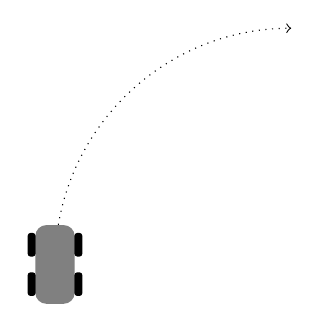
\begin{tikzpicture}
      
    \coordinate (start) at (0,0);
    \draw[->,dotted] (start) arc (180:90:3);

    \begin{scope}
      \node[ 
        fill=gray,minimum height=1cm, minimum width=0.5cm,rounded corners
        ] (car) at (0,0) {};
      \fill[rounded corners=1pt] 
        (car.east) ++(-0.01,0.1) rectangle ++(0.1,0.3);
      \fill[rounded corners=1pt] 
        (car.east) ++(-0.01,-0.1) rectangle ++(0.1,-0.3);
      \fill[rounded corners=1pt] 
        (car.west) ++(0.01,0.1) rectangle ++(-0.1,0.3);
      \fill[rounded corners=1pt] 
        (car.west) ++(0.01,-0.1) rectangle ++(-0.1,-0.3);
    \end{scope}

  \end{tikzpicture}
  \vs

\question
  The Indianapolis Motor Speedway has turns that are banked at 9.2~degrees.  The radius of curvature of these turns is 250 meters.  What is the maximum speed that a car can take around the curve so that no friction from the car's wheels is required?
  \vs[2]

\end{questions}



\end{document}